%%%%%%%%%%%%%%%%%%%%%%%%%%%%%%%%%%%%%%%%%%%%%%%%%%%%%%%%%%%%%%%%%%%%%%
% BAB METODOLOGI
%=====================================================================
\renewcommand{\thechapter}{\Roman{chapter}}
\addtocontents{toc}{\vskip10pt}
\chapter{METODOLOGI}
\renewcommand{\thechapter}{\arabic{chapter}}
%---------------------------------------------------------------------

%=====================================================================
\section{Diagram Alir Penelitian}
%=====================================================================

Dalam konteks penelitian ini, penting untuk menyadari bahwa pencapaian hasil yang berkualitas dan signifikan melibatkan proses yang terstruktur dan sistematis. Progres yang efektif dalam eksplorasi masalah penelitian didasarkan pada langkah-langkah yang diatur secara terencana dan berkesinambungan. Oleh karena itu, penelitian ini menjelaskan dan mengikuti serangkaian tahapan yang saling terkait, yang dirinci secara kronologis dan terurai dalam diagram alir yang dapat dilihat pada Gambar 3.1.

\begin{figure}
    \centering
    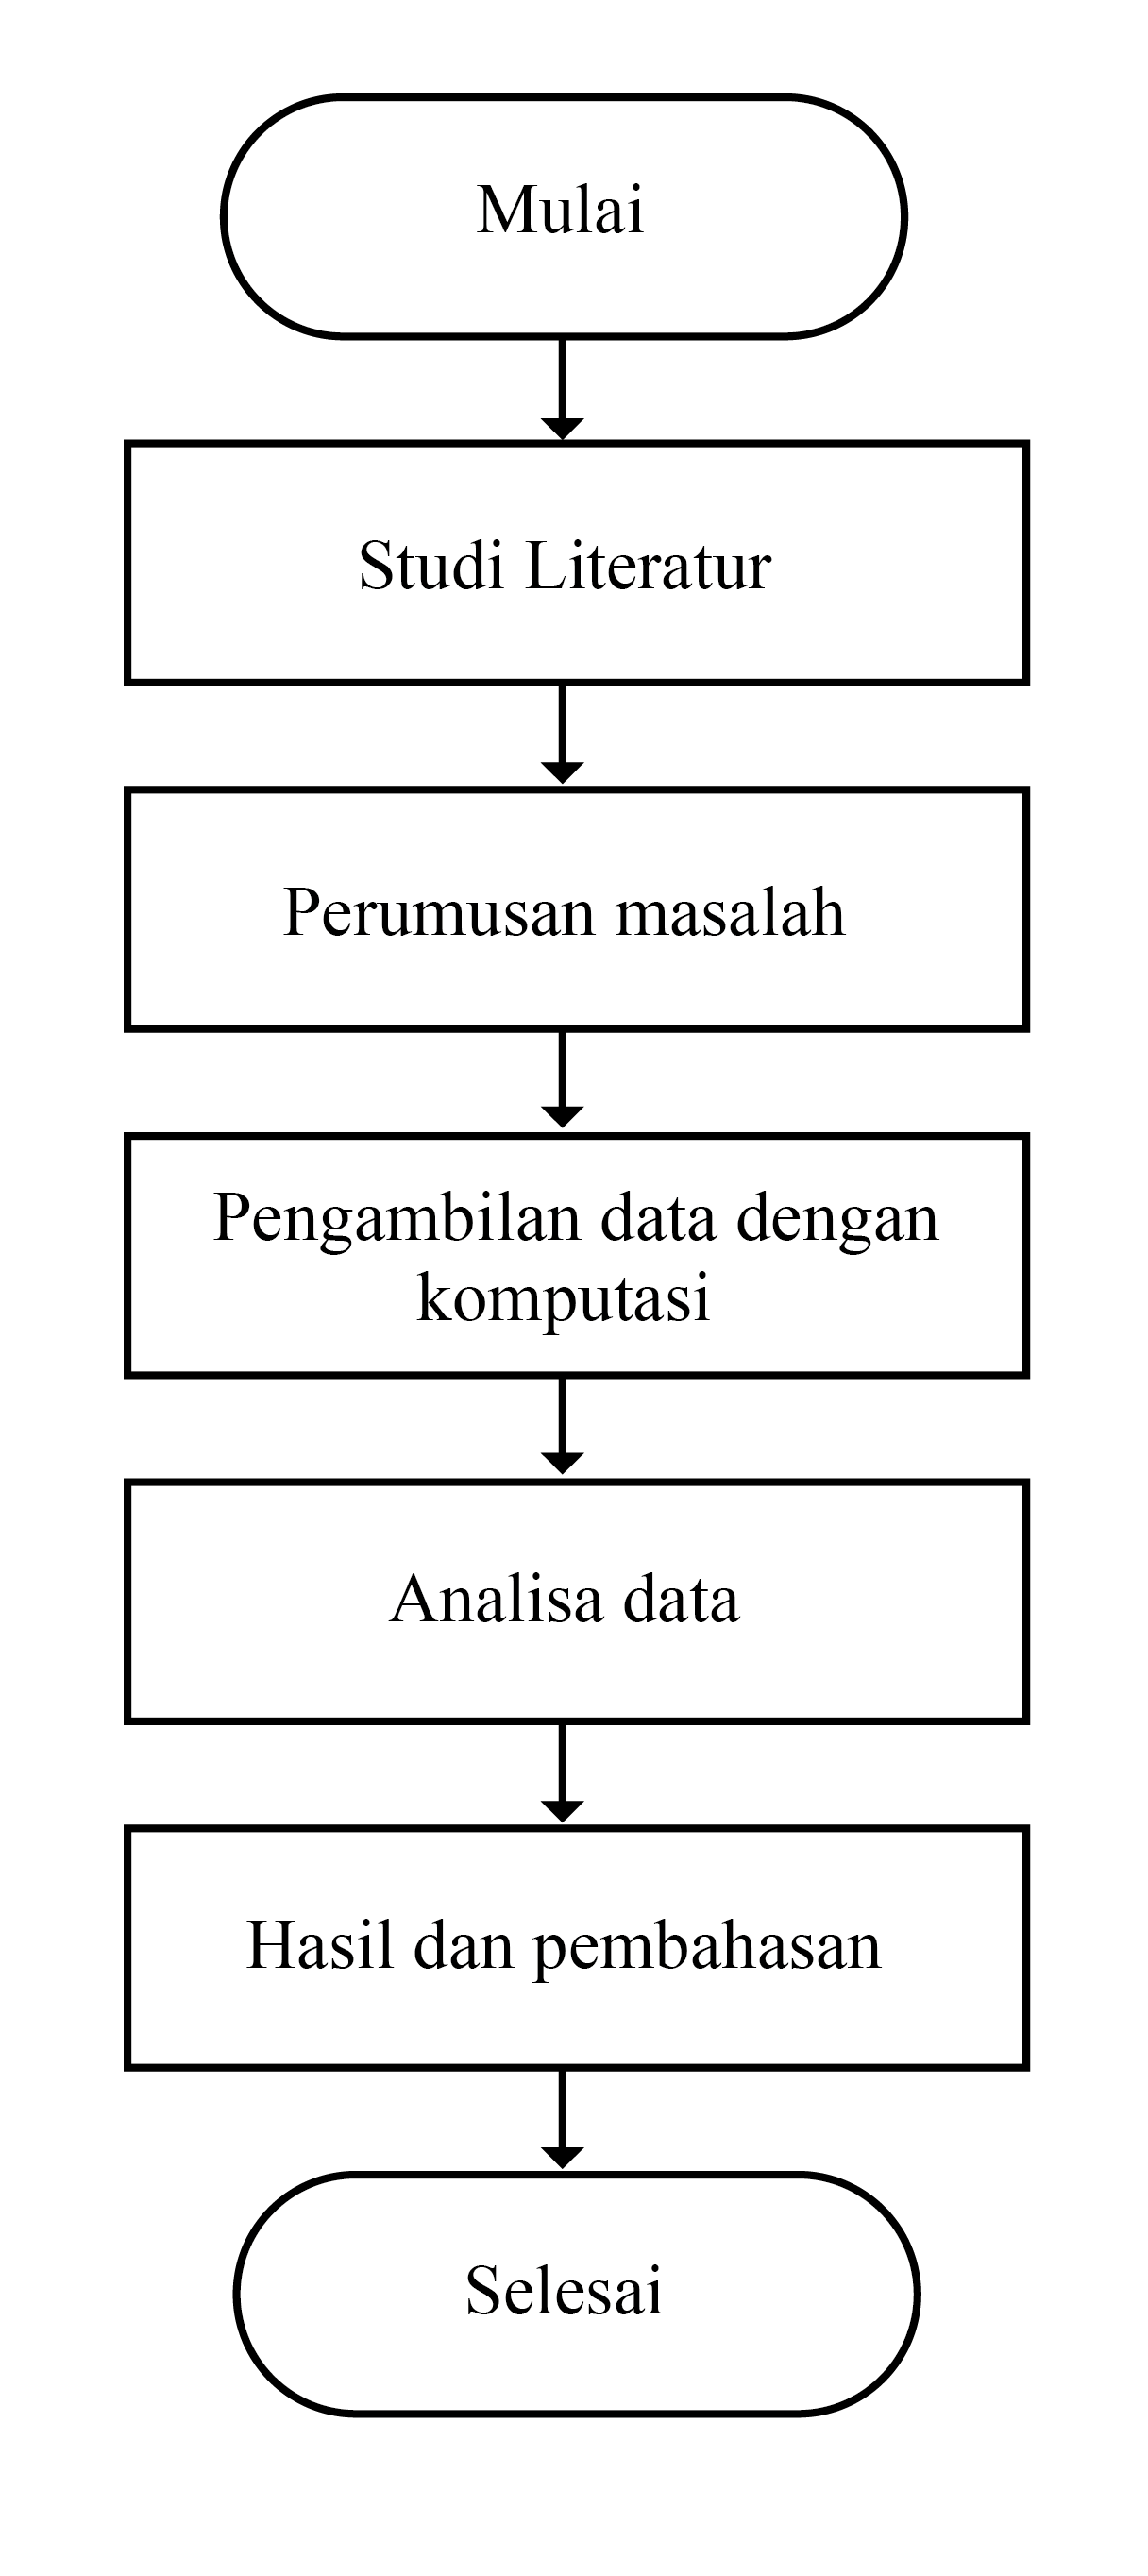
\includegraphics[width=5cm]{gambar/Flowchart Kegiatan.png}
    \caption{Diagram Alir Penelitian}
\end{figure}

%=====================================================================
\section{Jenis dan Desain Penelitian}
%=====================================================================
Pada penelitian ini jenis penelitian yang digunakan adalah penelitian komputasi, yaitu penelitian yang dilakukan di dalam komputer dengan metode pemodelan mekanika kuantum komputasi untuk menyelidiki sifat elektronik pada Stanene 2-dimensi menggunakan perangkat lunak Quantum ESPRESSO.


%=====================================================================
\section{Lokasi dan Waktu Penelitian}
%=====================================================================
Penelitian ini dilakukan pada saat melakukan kerja praktik
dan bimbingan di Pusat Riset Fisika Kuantum, Badan Riset dan
Inovasi Nasional (BRIN) yang berlokasi di Kawasan Sains dan Teknologi (KST) B. J. Habibie, Serpong, Tangerang Selatan. Waktu pelaksanaan tugas akhir selama 1 bulan (7 januari 2023 - 31 Januari 2023). 

%=====================================================================

%---------------------------------------------------------------------

\subsection{Perangkat Penelitian}
%---------------------------------------------------------------------
Pada penelitian ini menggunakan perangkat komputer berupa laptop yang dimiliki oleh peneliti

%---------------------------------------------------------------------
\subsection{Prosedur Penelitian}
Dalam prosedur penelitian ini, kami secara komprehensif membahas perangkat yang telah digunakan untuk mendukung jalannya penelitian ini, serta merincikan langkah-langkah kerja yang kami lakukan dalam rangka mencapai tujuan yang telah ditetapkan. Pada tahap awal, kami akan memberikan gambaran mendalam tentang perangkat keras dan perangkat lunak yang menjadi tulang punggung eksperimen ini. Ini mencakup spesifikasi teknis dari komputer yang digunakan untuk menjalankan perhitungan, perangkat pendukung seperti ketersediaan sumber daya komputasi berkecepatan tinggi, dan perangkat lunak yang mendukung analisis dan pengolahan data.

Selanjutnya, dalam upaya kami untuk mewujudkan simulasi yang akurat dan konsisten, kami akan memaparkan detail komputasi yang digunakan sebagai dasar input untuk program Quantum ESPRESSO. Ini melibatkan parameter-parameter yang terlibat dalam setiap perhitungan, termasuk energi kinetik \textit{cut-off}, ukuran grid \texttt{K-POINTS}, dan jenis potensial yang digunakan. Penjelasan rinci ini akan memberikan pemahaman mendalam tentang pemilihan parameter dan konfigurasi tertentu yang kami terapkan dalam eksperimen ini.

Langkah demi langkah, kami akan menggambarkan proses komputasi yang diterapkan, dari persiapan input hingga eksekusi perhitungan, serta tahap analisis hasil yang dihasilkan. Dengan memberikan informasi yang lengkap dan rinci tentang seluruh prosedur komputasi, kami berharap bahwa penelitian ini akan lebih mudah diulang oleh pihak lain dan menghasilkan hasil yang konsisten serta dapat diverifikasi. Dengan demikian, bagian ini tidak hanya akan memberikan panduan praktis bagi pembaca yang ingin mengulangi eksperimen, tetapi juga menguraikan landasan kuat dari eksperimen kami yang memanfaatkan alat Quantum ESPRESSO untuk mendapatkan wawasan yang berharga dalam ranah penelitian ini. 
%---------------------------------------------------------------------

\vspace{3mm}

\subsubsection{Detail Komputasi}
Dalam penelitian ini digunakan \qe  sebagai perangkat lunak komputasi\citep{Giannozzi_2009}. Kami gunakan sel satuan untuk membentuk struktuk \textit{stanene}. Dengan variasi \texttt{ecutwfc} sebesar 60 Ry dan \texttt{K-POINTS} sebesar $24\times24\times1$ untuk membagi daerah Brillouin dengan kisi Monkhorst Pack (MP)\citep{MP}. Kedua nilai tersebut diperoleh dari uji konvergensi yang akan dijelaskan lebih lengkap pada BAB 4. Digunakan fungsional Perdew-Burke-Ernzerhof (PBE)\cite{PBE} sebagai \textit{generalized gradient approximation} (GGA) untuk melengkapi fungsi korelasi dan pertukaran. Potensial semu yang digunakan untuk menggambarkan elektron valensi dan elektron inti adalah\textit{projector augmented wave method} (PAW)\citep{PAW}. Selain itu, ruang vakum dibuat sebesar .

Diagram alir komputasi yang akan dilakukan dalam penelitian ini dapat dilihat pada Gambar \ref{FlowchartKomputasi}. Seluruh prosedur komputasi dalam Gambar \ref{FlowchartKomputasi} dilakukan dalam \qe. Sementara visualisasi data hasil komputasi dibuat dengan bantuan dari kode python menggunakan library matplotlib dan numpy yang dibuat di dalam VS code dengan jupyter notebook.
\begin{figure}
    \centering
    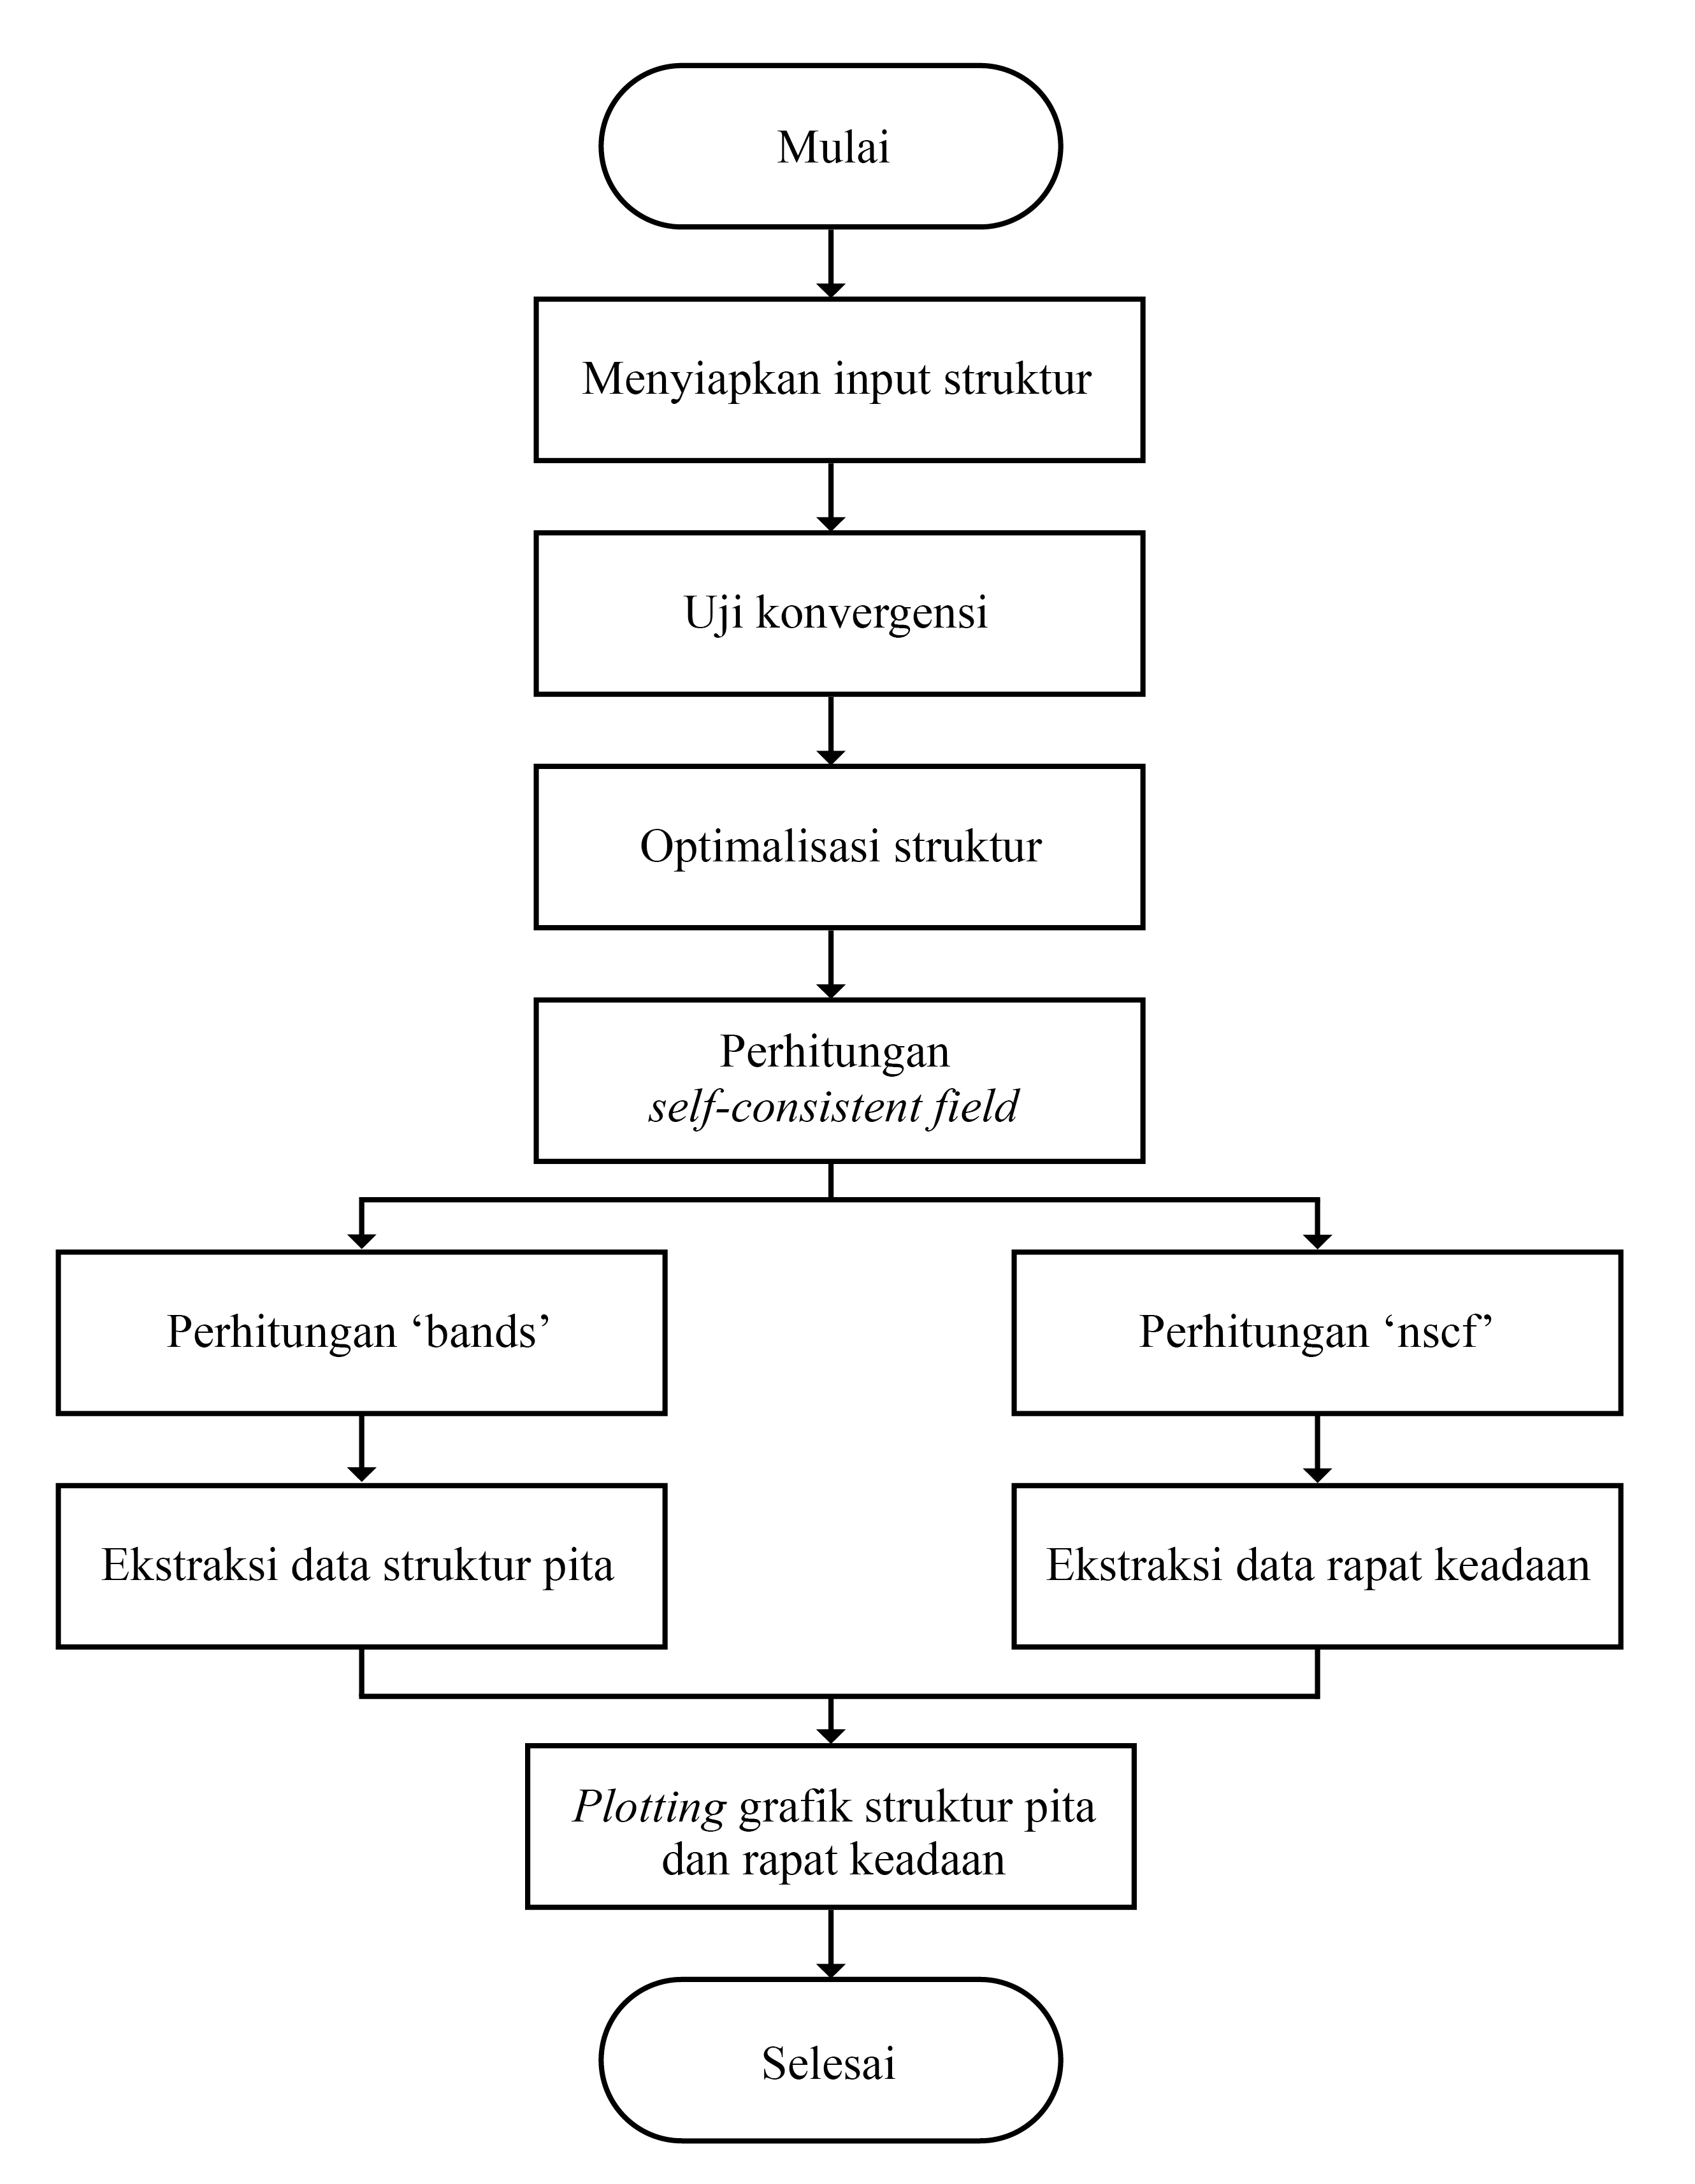
\includegraphics[width=12cm]{gambar/Flowchart Komputasi.png}
    \caption{Diagram alir komputasi}
    \label{FlowchartKomputasi}
\end{figure}

\subsubsection{Persiapan Struktur input}
Sebelum melakukan optimasi struktur, tentunya kita perlu membentuk material yang kita hendaki. Dalam penelitian ini terdapat 5 struktur yang akan dihitung sifat elektroniknya, dengan masing-masing struktur dijelaskan lebih lanjut di BAB 4. Untuk contoh kalkulasi dalam BAB ini, kami ambil struktur stanene. Secara garis besar ada 2 bagian penting dalam \textit{input} Quantum ESPRESSO yaitu \textit{Name Card}, dan \textit{Name List}. \textit{Name card} adalah file input utama dalam Quantum ESPRESSO yang mengandung semua informasi dasar tentang tugas perhitungan yang akan dilakukan. \textit{Name card} berisi informasi seperti tipe kisi, parameter elektronik, dan parameter lain yang spesifik untuk jenis perhitungan tertentu. Sedangkan \textit{Name list} adalah bagian dari \textit{name card} yang berisi kelompok parameter yang berhubungan dengan tugas perhitungan tertentu. \textit{Name list} dikelompokkan berdasarkan fungsinya dalam perhitungan. Misalnya, beberapa \textit{name list} yang umum dalam Quantum ESPRESSO adalah \texttt{CONTROL}, \texttt{SYSTEM}, \texttt{ELECTRONS}, \texttt{IONS}, dan sebagainya. Setiap namelist memiliki sejumlah parameter yang dapat disesuaikan untuk mengatur perilaku perhitungan.

File input stanene yang kami gunakan dapat dilihat sebagai berikut
\begin{lstlisting}
&control
calculation = 'scf'
prefix='stanene',
pseudo_dir = '../pseudo/',
outdir='../tmp/'
/
&system
ibrav = 4,
a=4.68
c=20,
nat = 2,
ntyp = 1,
ecutwfc = 60.0,
occupations = 'smearing'
smearing = 'm-p'
degauss = 0.02
/
&electrons
mixing_beta = 0.7
conv_thr = 1.0d-6
/
ATOMIC_SPECIES
Sn 118.710 Sn_pbe_v1.uspp.F.UPF
ATOMIC_POSITIONS (crystal)
Sn 0.333333333 0.666666666 0.500000000
Sn 0.666666666 0.333333333 0.500000000
K_POINTS {automatic}
24 24 1 0 0 0
\end{lstlisting}
input di atas merupakan input kalkulasi \texttt{scf}. Namelist \texttt{ibrav} berfungsi untuk mendefinisikan sistem kristal apa yang ingin kita gunakan. Dalam penelitian ini, kami menggunakan \texttt{ibrav}=4 yang mendefinisikan sistem kubik sebagai sel satuan. $a$, $b$, dan $c$ berturut-turut adalah besar vektor kisi pada arah sumbu $x$, $y$, dan $z$. Penentuan angka 4.68 dalam input diatas berdasarkan data parameter kisi stanene sebelumnya. Angka ini dipilih agar iterasi yang dilakukan tidak terlalu lama. Namelist \texttt{nat} mendefinisikan jumlah atom dalam sel yang kita bentuk sedangkan \texttt{ntyp} mendefinisikan berapa jenis atom dalam sel yang kita bentuk. namelist \texttt{ecutwfc} adalah energi kinetik \textit{cut-off} yang nilainya diperoleh melelaui uji konvergensi yang akan dijelaskan pada BAB selanjutnya.

\begin{table}[ht] % [h] menyatakan posisi. h: here, t: top, b: bottom
	\centering
	\caption{Kode-kode \texttt{ibrav} dalam Quantum ESPRESSO.}
	\label{tabel optimasi}
	\label{tab:ibrav}
\begin{tabular}{c c p{4cm} }
\hline
\textbf{Kode ibrav} & \textbf{Jenis Kisi} & \textbf{Sistem Kristal} \\
\hline
 1 & Kubik Primitif & $a=b=c$, $\alpha=\beta=\gamma=90^\circ$ \\
\hline
 2 & Kubik Berpusat pada Badan & $a=b=c$, $\alpha=\beta=\gamma=90^\circ$ \\
\hline
 3 & Kubik Berpusat pada Wajah & $a=b=c$, $\alpha=\beta=\gamma=90^\circ$ \\
\hline
 4 & Kubik Berpusat pada Ruang & $a=b=c$, $\alpha=\beta=\gamma=90^\circ$ \\
\hline
 5 & Tetragonal Primitif & $a=b\neq c$,  $\alpha=\beta=\gamma=90^\circ$ \\
\hline
 6 & Tetragonal Berpusat pada Badan & $a=b\neq c$,  $\alpha=\beta=\gamma=90^\circ$ \\
\hline
 7 & Ortorombik Primitif & $a\neq b\neq c$,  $\alpha=\beta=\gamma=90^\circ$ \\
\hline
 8 & Ortogonal Berpusat pada Badan & $a\neq b\neq c$,  $\alpha=\beta=\gamma=90^\circ$ \\
\hline
 9 & Ortogonal Berpusat pada Wajah & $a\neq b\neq c$, $\alpha=\beta=\gamma=90^\circ$ \\
\hline
 10 & Rhombohedral & $a=b=c$,  $\alpha=\beta=\gamma\neq90^\circ$ \\
\hline
 11 & Monoklinik Primitif & $a\neq b\neq c$,  $\alpha=\gamma=90^\circ, \beta\neq90^\circ$ \\
\hline
 12 & Monoklinik Berpusat pada Badan & $a\neq b\neq c$, $\alpha=\gamma=90^\circ, \beta\neq90^\circ$ \\
\hline
 13 & Trigonal Primitif & $a=b=c$, $\alpha=\beta=\gamma\neq90^\circ$ \\
\hline
 14 & Trigonal Berpusat pada Badan & $a=b=c$, $\alpha=\beta=\gamma\neq90^\circ$ \\
\hline
 15 & Trigonal Berpusat pada Wajah & $a=b=c$, $\alpha=\beta=\gamma\neq90^\circ$ \\
\hline
	\end{tabular}
\end{table}

Pada \texttt{ATOMIC\_SPECIES} terdapat jenis atom yang menyusun sel satuan yang kita bentuk, dalam hal ini untuk struktur stanene maka atom penyusun pad struktur hanyalah atom timah (Sn). Di samping lambang unsur, terdapat massa atom yang juga perlu didefinisikan serta \textit{pseduopotential} (potensial semu) yang akan digunakan. File \textit{pseudopotential} disimpan dalam direktori khusus agar mudah dipanggil dalam perhitungan untuk struktur lainnya.

\subsubsection{Uji Konvergensi}
Uji konvergensi adalah proses penting dalam perhitungan menggunakan paket perangkat lunak Quantum ESPRESSO untuk memastikan bahwa hasil perhitungan numerik sudah cukup akurat dan stabil. Ada dua parameter utama yang sering diuji untuk konvergensi \texttt{ecutwfc} dan \texttt{kpoints}. Parameter \texttt{ecutwfc} (\textit{energy cut-off for wave functions}) adalah nilai energi maksimum yang digunakan untuk memotong fungsi gelombang elektron. Nilai ini menentukan sejauh mana deret Fourier digunakan untuk merepresentasikan fungsi gelombang. Semakin tinggi nilai \texttt{ecutwfc}, semakin banyak komponen deret Fourier yang digunakan, yang pada gilirannya dapat meningkatkan akurasi hasil perhitungan. Sedangkan titik-titik k (\texttt{K-POINTS}) digunakan untuk menghitung integral di dalam ruang resiprok. Jumlah dan distribusi titik-titik k memiliki dampak pada akurasi hasil perhitungan, terutama untuk sifat-sifat terkait permukaan energi, densitas elektron, dan lainnya. Dalam penelitian ini, dilakukan siklus \texttt{scf} seperti yang ditampilkan dalam skema diagram alir 3.3, kami melakukan perhitungan dengan mencoba beberapa variasi \texttt{ecutwfc} dan melihat di nilai \texttt{ecutwfc} berapakah energi sistem mulai konvergen. Hal serupa dilakukan untuk menemukan konvergensi nilai \texttt{K-POINTS}.


\subsubsection{Optimasi Struktur}
Nilai konstanta kisi dan posisi atom dalam struktur input bukanlah posisi paling optimal. Oleh karena itu kita perlu melakukan relaksasi strukutur dengan menggunakan perintah kalkulasi \texttt{vc-relax}. \texttt{vc-relax} (\textit{Variable Cell Relaxation}) adalah kalkulasi untuk merelaksasi struktur kristal. Tujuan utamanya adalah untuk mencari konfigurasi struktur yang memiliki minimum energi total minimum, yang menggambarkan keadaan terstabilkan dari sistem kristal yang kita miliki.

Untuk melakukan kalkulasi \texttt{vc-relax}, input file Quantum ESPRESSO pada bagian \texttt{calculation} perlu didefinisikan sebagai
\begin{lstlisting}
calculation = 'vc-relax'
\end{lstlisting}

\begin{figure}
    \centering
    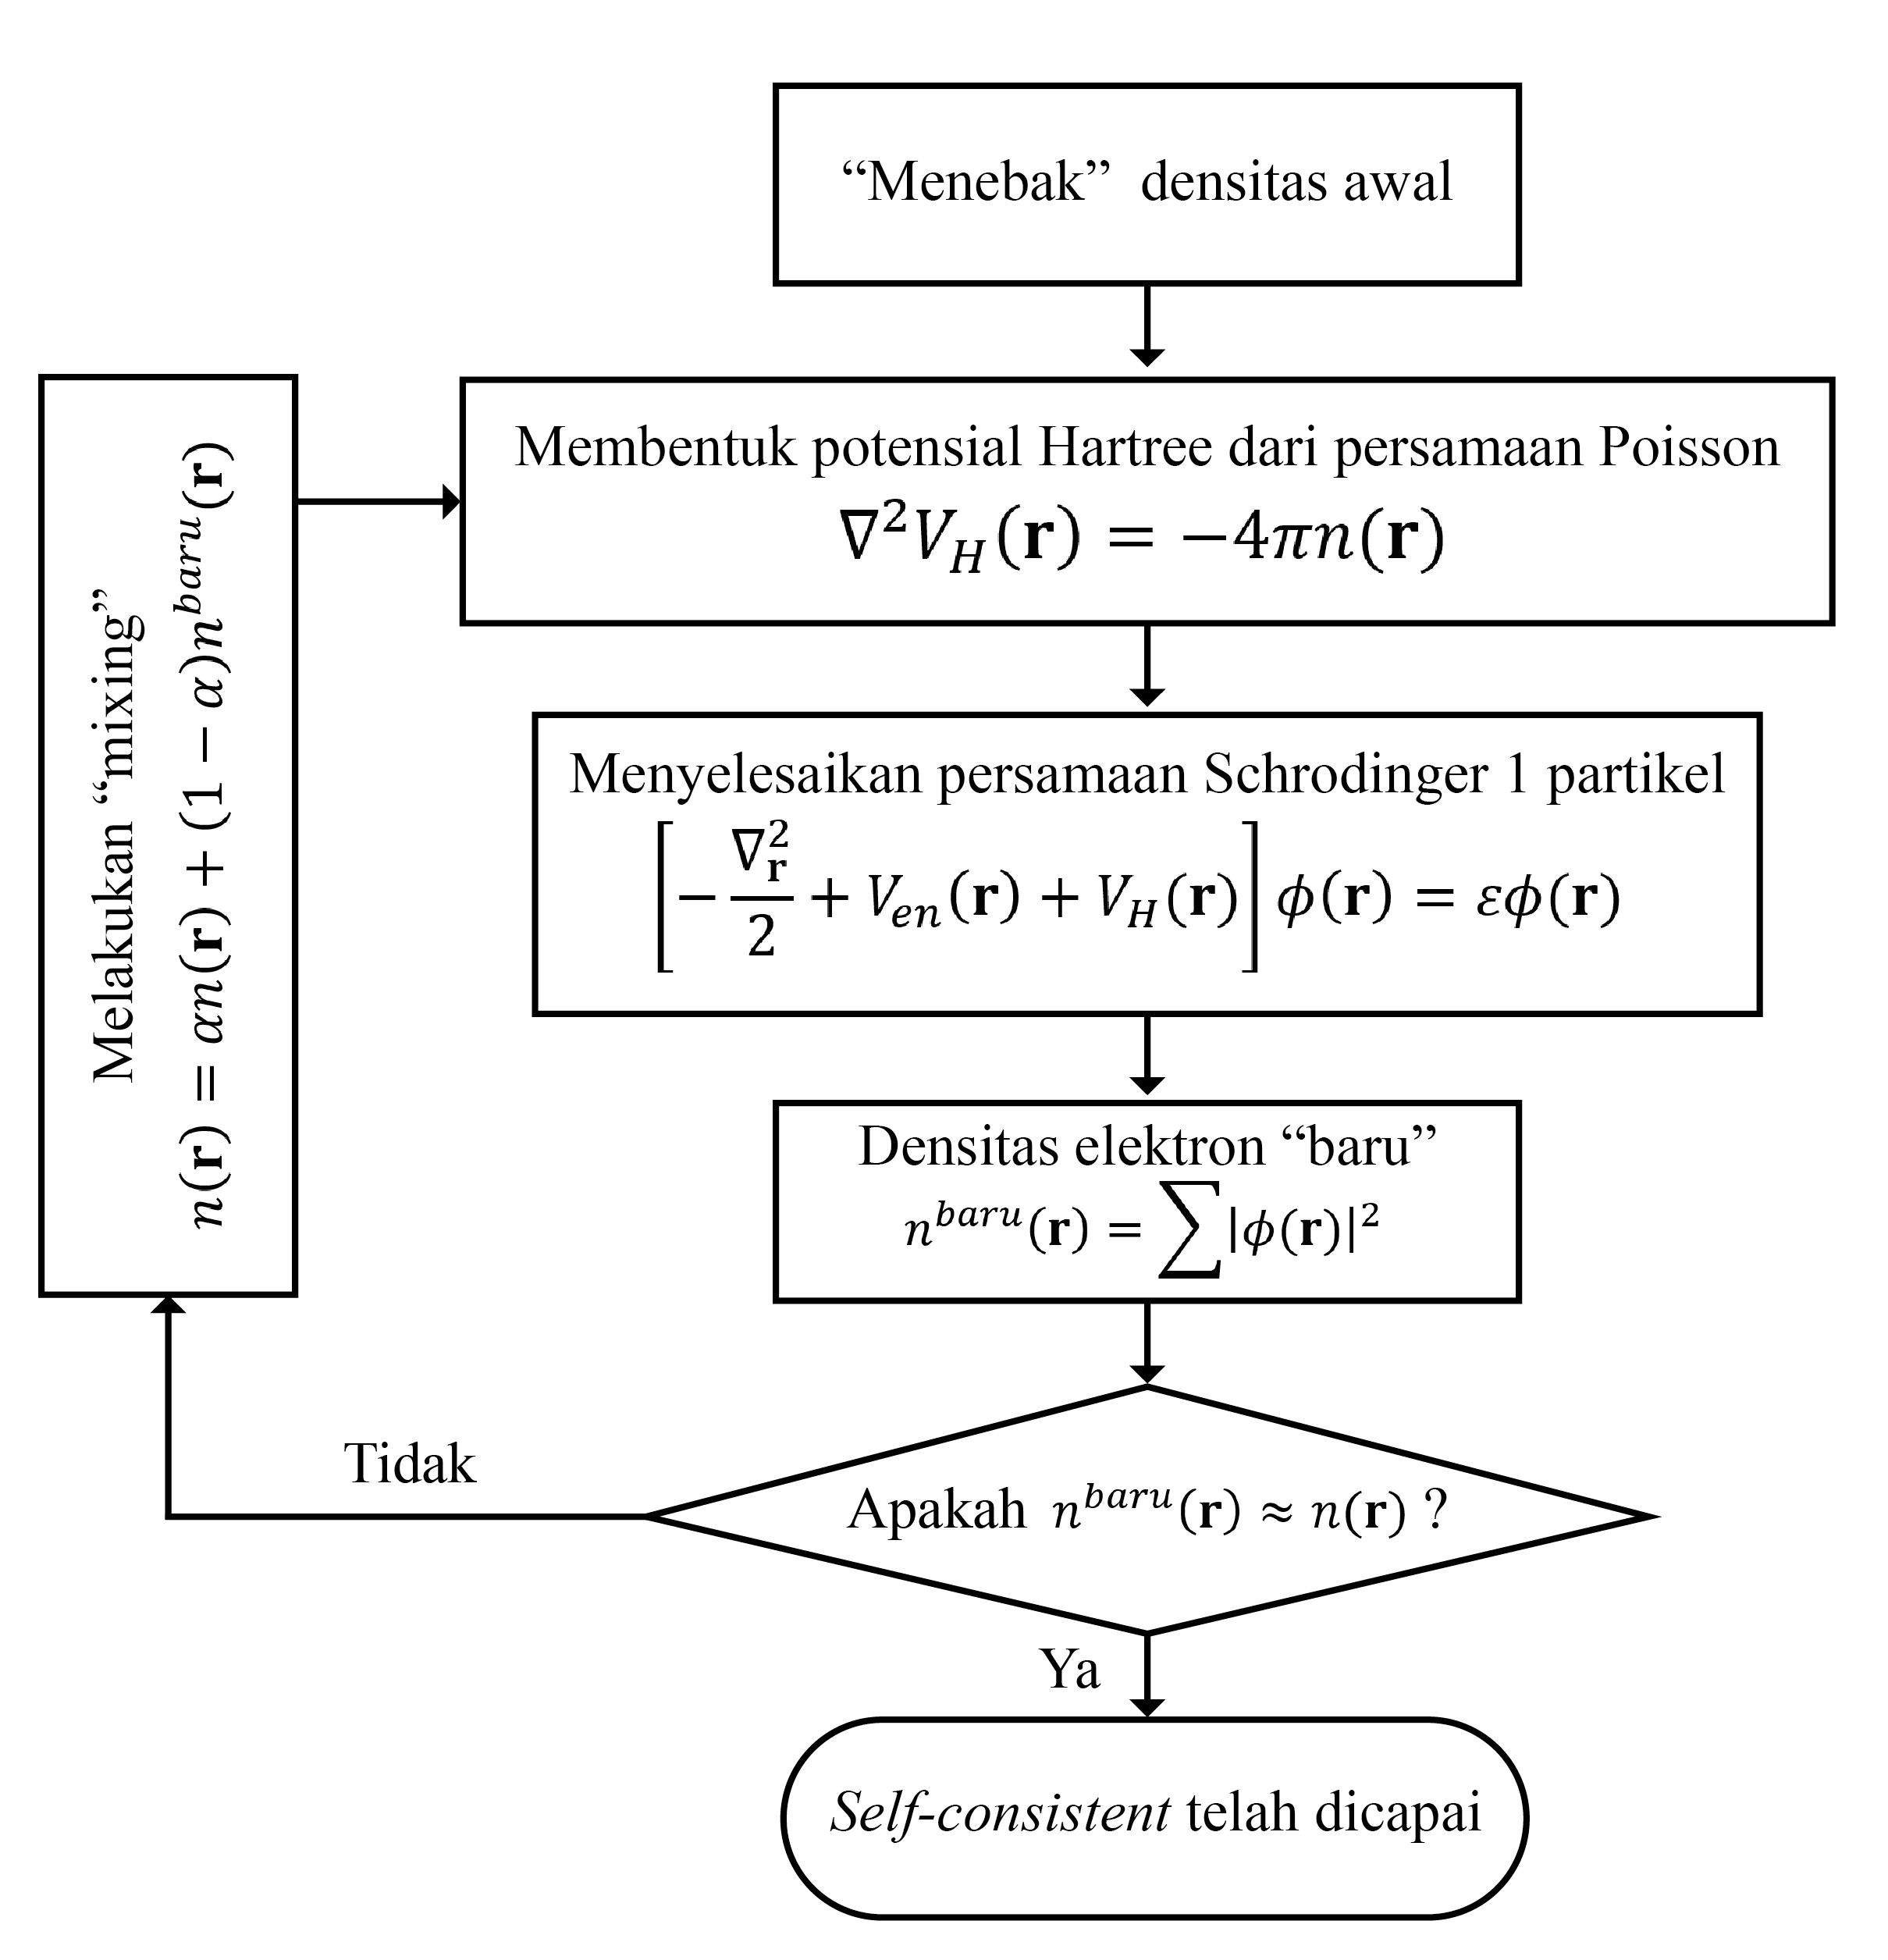
\includegraphics[width=12cm]{gambar/Flowchart SCF.png}
    \caption{Siklus kalkulasi \textit{self-consistent field}.}
    \label{fig:SCF}
\end{figure}
Prinsip perhitungan nilai energi yang digunakan ialah dengan skema \texttt{scf}. Skema ini dapat dilihat pada Gambar \ref{fig:SCF} Perhitungan dilakukan dengan memberikan potensial inti yang dikonstruksi, dimana dalam Quantum ESPRESSO potensial ini ditentukan oleh \textit{pseudopotential} yang didapatkan dari \textit{library} Quantum ESPRESSO. Tebakan awal dari kerapatan berasal dari atom-atom yang digunakan, yang selanjutnya akan digunakan untuk menghitung potensial Hartree dan potensial \textit{exchange-correlation}. Potensial efektif merupakan gabungan antara potensial inti, Hartree dan \textit{exchange-correlation} yang dimasukan di dalam persamaan Kohn-Sham. \textit{Output} dari persamaan menjadi \textit{input} dakam iterasi kembali hingga siklus ini mencapai \textit{self-consistent}. Kondisi \textit{self-consistent} ini terjadi saat kerapatan elektron hasil persamaan Khon-Sham dengan nilai kerapatan awal. Nilai kerapatan ini merupakan kerapatan pada kondisi \textit{ground-state} untuk mendapatkan energi sesuai dengan teorema Hohenberg-Kohn, namun jika \textit{self-consistent} tidak tercapai maka perlu dilakukan konstruksi fungsi kerapatan yang baru dan dilakukan iterasi kembali.

Perhitungan \texttt{scf} akan terus dilakukan hingga sistem berada pada keadaan yang paling stabil, yaitu keadaan dengan nilai energi terendah. Setelah file input dijalankan dengan perintah,
\begin{lstlisting}
    mpirun -np 6 pw.x  < vc-relax.in > vc-relax.out
\end{lstlisting}
akan diperoleh file output graphene.relax.out yang menginformasikan koordinat atom dan parameter kisi yang sudah teroptimalisasi seperti berikut

\begin{lstlisting}
    Begin final coordinates
     new unit-cell volume =   2563.91358 a.u.^3 (   379.93279 Ang^3 )
     density =      1.03767 g/cm^3

CELL_PARAMETERS (alat=  8.84391826)
   1.000753744   0.000000000   0.000000000
  -0.500376872   0.866678165   0.000000000
   0.000000000   0.000000000   4.273504274

ATOMIC_POSITIONS (crystal)
Sn            0.3333333330        0.6666666660        0.5000000000    
Sn            0.6666666660        0.3333333330        0.4579351681
\end{lstlisting}
output di atas merupakan koordinat optimal dari stanene yang digunakan dalam penelitian ini. Terlihat bahwa kita diberikan dua parameter yaitu \texttt{CELL\_PARAMETERS}, dan \texttt{ATOMIC\_POSITIONS}. Nilai inilah yang akan kita gunakan untuk melakukan perhitungan lanjut seperti struktur pita dan rapat keadaan. Perlu diingat bahwa secara praktis kita tidak perlu memasukkan \texttt{CELL\_PARAMETERS} ketika kita mendefinisikan \texttt{ibrav} = 4.

\subsubsection{Perhitungan Struktur Pita}
Perhitungan struktur pita dilakukan dengan 3 file input, yang pertama adalah file input kalkulasi \texttt{scf}, kedua adalah kalkulasi \texttt{bands}, dan terakhir adalah file input untuk mengekstrak data struktur pita. File input \texttt{scf} pada perhitungan struktur pita sama dengan file input \texttt{scf} sebelumnya, namun pada \texttt{name card} \texttt{SYSTEM} perlu ditambah \textit{name list} \texttt{nbnd} yang mana namelist ini diperlukan untuk visualisasi jumlah keadaan yang ingin ditinjau.
\begin{lstlisting}
nbnd    = 16
\end{lstlisting}
kemudiaan file input \texttt{scf} dapat dijalankan dengan perintah
\begin{lstlisting}
mpirun -np 6 pw.x  < scf.in > scf.out
\end{lstlisting}

File kedua yaitu file yang serupa dengan file \texttt{scf} namun kita hanya mengganti \texttt{calculation} menjadi \texttt{'bands'}, dan mendefinisikan \texttt{K\_POINTS} secara lebih spesifik. Jika sebelumnya \texttt{K\_POINTS} mendefinisikan berapa jumlah grid untuk membagi daerah Brilloiun, di kalkulasi \texttt{bands} kita mendefinisikan \texttt{K\_POINTS} menjadi koordinat titik-titik \textit{high-symmetry point} seperti berikut.
\begin{lstlisting}
K_POINTS (crystal_b)
 4
 gG 40
 K 20
 M 30
 gG 0
\end{lstlisting}
dalam input di atas, jalur (\textit{k-path}) yang kita tentukan dari berawal titik $\Gamma$, K, M, dan $\Gamma$. Angka-angka di samping koordinat \textit{high-symmetry point} adalah perintah untuk membagi jalur (k-path) menjadi beberapa titik. Misal pada titik $\Gamma$ ke titik K, kita membagi jalur ini menjadi 50 titik yang akan dihitung dalam kalkulasi \texttt{bands}.

Langkah terakhir adalah mengekstraksi data perhitungan \texttt{bands} dari kalkulasi sebelumnya. Kita siapkan file input sebagai berikut
\begin{lstlisting}
&BANDS
 outdir  = '../tmp/'
 prefix  = 'stanene'
 filband = 'stanene.bands'
/

\end{lstlisting}
kemudian input ini dijalankan dengan perintah
\begin{lstlisting}
mpirun -np 6 bands.x < bands.in > bands.out
\end{lstlisting}
setelah \texttt{JOB DONE}, kita akan memperoleh file dengan format '.gnu'. File tersebut berisi dua kolom yang masing-masing memberikan nilai energi dan koordinat energi  tersebut dalam ruang vektor. File tersebut bisa lansung di-\textit{plot} menggunakan matplotlib.

\subsubsection{Perhitungan Rapat Keadaan (\textit{Density of States})}
Sama seperti perhitungan struktur pita, dalam perhitungan rapat keadaan, kita juga perlu file input \texttt{scf}. Namun 2 hal yang berbeda di sini adalah file kalkulasi '\texttt{nscf}' dan file input ekstraksi data-nya. Sebelumnya, dalam perhitungan \texttt{scf}, fungsi gelombang Kohn-Sham dan densitas elektron diterapkan untuk mencapai kondisi kesetimbangan, di mana potensial efektif dan densitas konvergen. Namun, hasil \texttt{scf} hanya memberikan informasi tentang struktur dasar elektronik dari sistem.

Perhitungan \texttt{nscf} dilakukan dengan mempertahankan struktur geometri dan densitas elektron yang telah dihasilkan dari perhitungan \texttt{scf}, tetapi mengubah beberapa parameter, seperti jumlah \texttt{K-POINTS} atau mesh dalam ruang k (\textit{k-space}), dan mendapatkan spektrum energi lebih lengkap di sekitar titik-titik tertentu di dalam zona Brillouin. Jadi misalnya di \texttt{scf} sudah diperoleh fungsi gelombang, maka di \texttt{nscf} akan diiterasi dengan interpolasi yang lebih rapat. File input \texttt{nscf} persis sama dengan \texttt{scf}, hanya saja kita merubah bagian \texttt{calculation} menjadi \texttt{'nscf'} seperti berikut.
\begin{lstlisting}
calculation = 'nscf'
\end{lstlisting}
kemudian pada \textit{name cards} \texttt{CONTROL} ditambahkan \texttt{verbosity = 'high'}, dan pada \texttt{SYSTEM} ditambahkan \texttt{"occupation = tetrahedra"}. Jenis \texttt{occupation} yang kita pilih berpengaruh pada bentuk rapat keadaan yang dihasilkan.
Berdasarkan penelitian sebelumnya \citep{toriyama2021comparison}, diketahui bahwa occupation jenis tetrahedra memberikan data yang lebih akurat untuk perhitungan rapat keadaan dibanding jenis \texttt{occupation} lain, seperti \texttt{gaussian}.

File ekstraksi data dos adalah
\begin{lstlisting}
&DOS
outdir = '../tmp'
prefix = 'stanene'
fildos = 'stanene.dos'
/
\end{lstlisting}
berbeda dengan \texttt{bands} output dari perhitungan \texttt{dos} adalah file dengan format '.dos' file ini berupa data dos yang siap di-\textit{plot} menggunakan matplotlib.